\documentclass[a4paper,12pt]{article}
\usepackage{mypackages}

\begin{document}
\section{Calculating the start of spring}
In order to properly calculate at which date spring starts, a 
definition for the season is necessary. On the webpage of SMHI 
(https://www.smhi.se/kunskapsbanken/meteorologi/var-1.1080)
a meteorological definition of spring is given. Below is the 
definition of the start of spring from SMHI.

\hfill\begin{minipage}[c]{\textwidth-2cm}
	If the daily average temperature is above 0 $^\circ$C but below 10 
	$^\circ$C, we call this for a day with spring temperature. If this 
	occurs seven days in a row,	we say that spring arrived the first of 
	these days. Even if there is a return to lower temperatures then it is
	still counting as spring.
	\newline
	$\ldots$
	\newline
	The start of spring can not occur before the 15th of febuary.
	\newline
	$\ldots$
	\newline
	Spring can, at latest, occur the 31th of July.
\end{minipage}

\noindent Using this definition, the temperature for spring arrival was 
extracted from the data. The method for reading, extracting, plotting, 
and, fitting the data is performed in a single method. There exist 
several ways to implement a solution of the posed question of spring 
arrival. The choice of using a single method is one of them. The inital 
set of lines of "springArrive()" initialize variables that will be used 
when reading the data file "uppsala\_tm\_1722-2013.dat".
\\\indent
The exact date for when each season start and end are not fixt and may 
vary a lot between each year. Using only the first paragraph of the 
above definition dates as late as november could be classified as the 
beginning of spring. For this reason, we use the last of July as a 
cutoff point. The beginning of spring may change a lot depending on 
location. The definition used here was found most promising for the 
data set of Uppsala. 

The main part of the springArrive() method occur in the while loop. It 
can be summarized in two parts. First check if the spring of the 
current year is found using the foundSpring variable. If foundSpring is 
true, the current year is extracted and the file pointer is moved down 
the file till it finds the next year. Note that when this loop is 
complete the the next line read will represent the earliest date
of next year given in the data file.

\begin{lstlisting}
if(foundSpring == true)
	{
		dayCount = 0;
		foundSpring = false;
		Int_t nextYear = year+1;
		while(nextYear != year)
		{
			if(getline(file,line, '\n'))
			{
				stringstream ssNextYear(line);
				ssNextYear >> year >> month >> day >> temp >> temp_urban >> id; 
			}
			else
				break;
		}
	}
\end{lstlisting}
If foundSpring is false, the file pointer is pointing at a year which 
has not yet been registered. In this case the second loop is used. 
Here, the program try performing a for loop representing the 7 day span 
required by the definition above. The id of the data is checked with 
the provided "dataset" variable so to  ensure only data from the 
correct data set is stored. Next, the temperature is examined, it has 
to be between 0 $^\circ$C and 10$^\circ$C. dayCount represent the 
total number of dates iterated of the year, regardless of id number. 
This ensures that spring will be identified even if data points might 
be missing. As a final requirement, the month can not exceed July, in 
line with the definition of SMHI. At the final iteration of the for 
loop, the first registered date and temperature is stored. Note the 
method does not divide the year into 52 weeks but instead look for the 
first 7 succeeding iterations which satisfy the definition we use.
\begin{lstlisting}
if(foundSpring == false)
	for(Int_t i=0; i < daysWeek; i++)
		{
			Double_t tmp;
			getline(file,line, '\n');
			stringstream ss(line);
			if(ss >> year >> month >> day >> temp >> temp_urban >> id) //check output can is eligible
			{
				dayCount++;
				if(id==dataset)//Take data from dataset
				{
					//dayCount>=46 represent 15 feb (minimum date for spring), month<8 
					remove missing data (otherwise autumn is classified as spring)
					if(temp_urban >= 0 && temp_urban <= 10 && dayCount >= 46 && month 
					< 8) //Check if temperature fulfill definition of spring
					{
						if(i==0)
						{
							sYear=year; sMonth=month; sDay=day;
							sTemp=temp_urban;
						}
						if(i == daysWeek-1) //Save temp of first day
						{
							foundSpring = true;
							hDays->Fill(dayCount - (daysWeek+1)); //(daysWeek+1), 
							+1 because dayCount incremented by 1 previously
							hTemp->Fill(sTemp);
							//Print date of spring
							cout << "Spring found:\t" << sYear << "\t" << sMonth << "\t" << sDay << "\t" << sTemp << endl;
							springDate << sYear << "\t" << sMonth << "\t" << sDay << "\t-\t" << sTemp << endl;
						}
					}
					else //If temperature is not in interval, start new iteration
						break;
				}
			}
		}
\end{lstlisting}
The date of each spring found is stored in a file 
"found\_spring\_date.dat". The registered days are saved in a histogram 
that span one year. The resulting histogram can be seen in figure 
\ref{fig:SA_dayHist}. Note the sharp start at day 46, representing the 
15th of february. The mean of the histogram, day 80, represent the 21 
of March if its not a leap year and the 20 of March otherwise. A total 
of 365 bins are used. One for each day, as seen on the x-axis, and, the 
y-axis represent the number of entries. For each date registered, the 
temperature is saved in a histogram, see figure \ref{fig:SA_tempHist} 
for more details. Here, the x-axis represent the temperature interval 
and the y-axis the number of entries. The resulting histogram is fitted 
to a exponential function,
\begin{equation}
	f(x)=\alpha e^{-\lambda x}.\label{eq:SA_fitfunc}
\end{equation}
The curve fit relatively well with the histogram. This is expected as 
the gradual increase of the temperature each spring should result in 
the majority of temperatures ending up in the low temperature region.
\begin{figure}[htb]
	\centering
	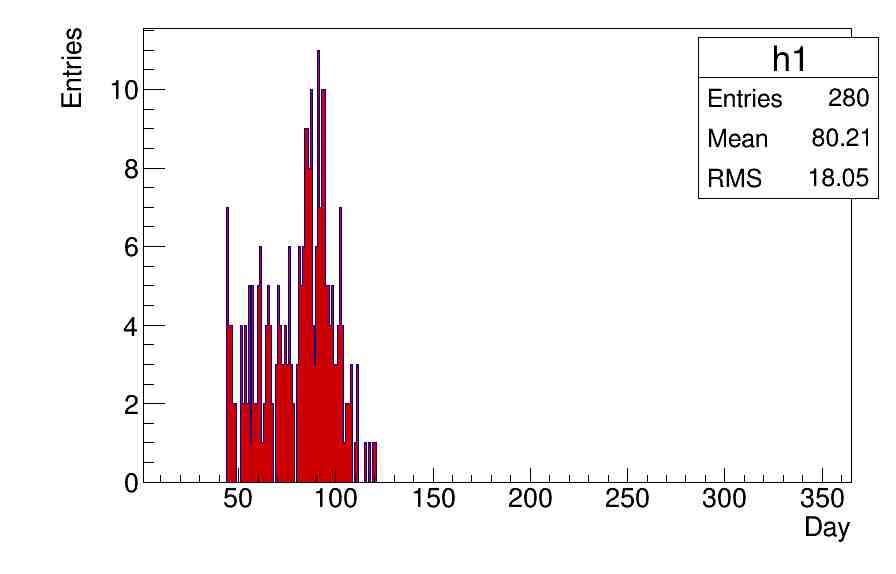
\includegraphics[scale=.4]{../Code/springArrive_dayHist.jpg}
	\caption{Number of times spring has arrived since the 18th century 
	in Uppsala using the meteorological definition of SMHI. Day 80, 
	, the mean of this histogram, represent either March 20 if its a 
	leap year or March 21 if its not a leap year. Note the sharp peak at 
	day 46, representing the 15th of febuary. Dates after the last of July  
	are not included. The histogram consist of 365 bins, one for each day 
	of the year, seen on the x-axis, and, the number of entries on the 
	y-axis. This binning shifts leap years by one day, however the 
	effect is neglectable.}
	\label{fig:SA_dayHist}
\end{figure}
\begin{figure}[htb]
	\centering
	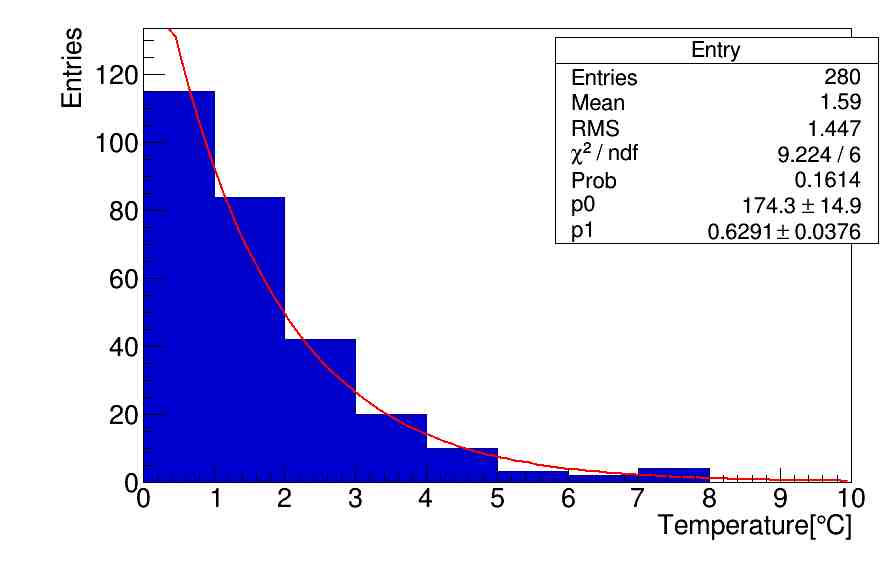
\includegraphics[scale=.4]{../Code/springArrive_tempHist.jpg}
	\caption{Temperature histogram for all spring arrival dates (blue) and 
	fitted exponential function (red line), see equation 
	\eqref{eq:SA_fitfunc}. The histogram fit relatively well with a 
	exponential function, as expected since the gradual increase of the 
	temperature each year should yield a decaying distribution. Here, 
	$p0$ represent $\alpha$, and, $p1$ represent $\lambda$ of equation 
	\eqref{eq:SA_fitfunc}. The x-axis represent the temperature in 
	$^\circ$C and the y-axis the number of entries.}
	\label{fig:SA_tempHist}
\end{figure}
\end{document}
